ユーザとシステムが行う対話は大きく分けると,タスク指向型対話と雑談対話の 2 種類が存在する.タスク指向型対話とは,ユーザが特定の目的を持ち,ユーザとシステムが応答を繰り返すことでその目的を達成する対話のことである.雑談対話とは,対話そのものを目的として行うもので,明確な目的が存在しない対話のことである.また,前章で述べた一問一答型の対話はタスク指向型対話の一部で,対話状態を用いずに一回の応答でユーザの要求に応える対話のことである.一問一答型の対話は一回の応答で対話が完結するため,ユーザの細かい要求に応えられないという問題がある.
\par
タスク指向型対話システムとは,タスク指向型対話を行う対話システムのことであり,ホテル案内,レストラン案内,交通案内など様々なドメインを扱う.タスク指向型対話システムの実用例として,バス案内システムとして実運用されている「Let's Go システム」\cite{letsgo} や大学のキャンパス案内を行う「正門メイちゃん」\cite{mmdagent}が挙げられる.
\par
\begin{figure}[thb]
  \centering
  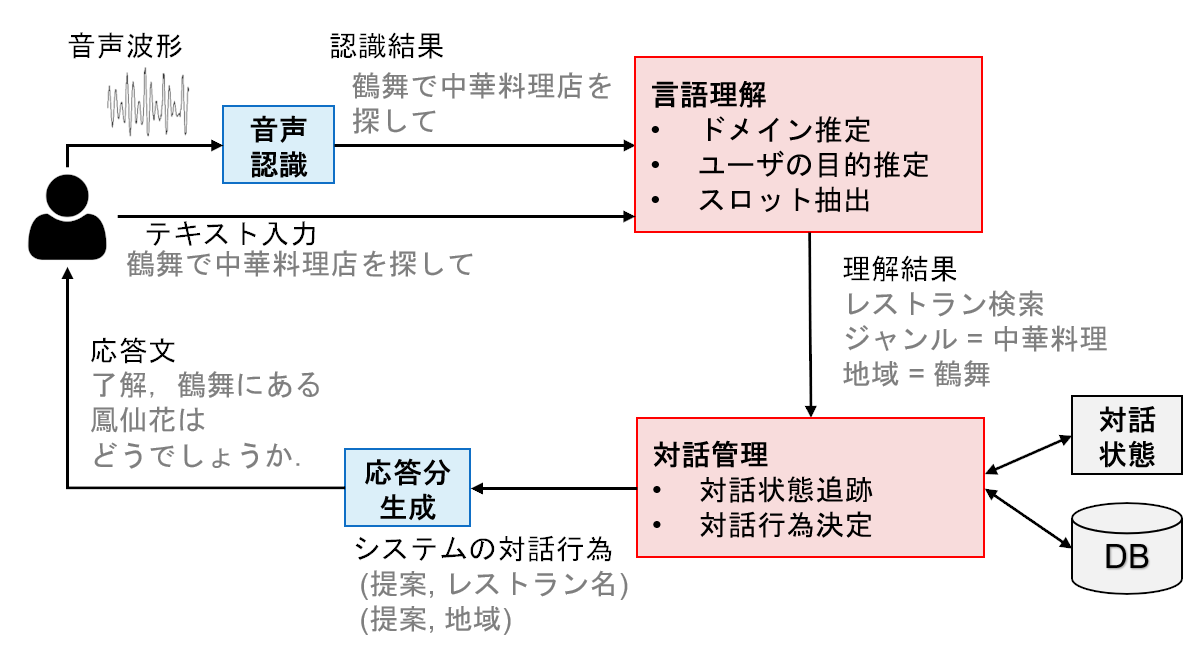
\includegraphics[width=15cm]{chapter2/system3.eps}
  \caption{タスク指向型対話システムの基本構成}
  \label{fig:taiwasystem}
\end{figure}
タスク指向型対話システムの基本構成を図\ref{fig:taiwasystem}に示す.対話システムは大きく分けて,音声認識部,言語理解部,対話管理部,応答生成部の4つのモジュールで構成されている.音声認識部はユーザの発話音声を認識し発話文に変換し,言語理解部はその発話文をシステムが理解できる形に変換する部位である.言語理解部が行うことは,発話文からユーザが行おうとしているタスクのドメインが何か推定するドメイン推定,そのドメイン中でのユーザの目的は何か推定するユーザの目的推定,発話中に含まれるスロットの値候補を見つけるスロット抽出の 3 つである.スロットとはドメインごとに与えられる属性のことで,システムはスロットと値の組によってユーザの要求を表現する.そして対話管理部は,過去の発話も考慮してユーザの目的と要求を推定する対話状態追跡と,対話状態から不足している情報を検出し次のシステムの行動を決定する対話行為決定を行う.最後に,応答文生成部でシステムの対話行為に沿った応答文を生成する.このようにタスク指向型対話システムは,4つのモジュールでユーザとのタスク指向型対話を可能にする.
